\subsubsection{Manually pull up \texttt{TX\_RDY}}
DCB pilot boards have a design flaw that prevents them pulling up
\texttt{TX\_RDY} automatically.
This would prevent PRBS tests, since without it pulling up, MiniDAQ would
consider data frames as ``invalid''\footnote{
    Which is not really the case, as all \texttt{TX\_RDY} does is flip single
    bit 0 to 1 on the header part of the data frame.
}.

A large ($\approx$ 5~k$\Omega$) resistor is connected to the \emph{data GBTx}
FFC breakout boards.
See \autoref{fig:dcb_tx_rdy_pull_up} for connection details.

\begin{figure}[!ht]
\centering
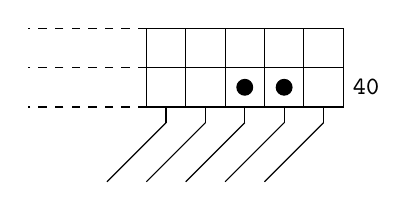
\begin{tikzpicture}
    % Pins
    \draw (0,0) rectangle (0.5,0.5);
    \draw (0.5,0) rectangle (1,0.5);
    \draw (1,0) rectangle (1.5,0.5);
    \draw (1.5,0) rectangle (2,0.5);
    \draw (2,0) rectangle (2.5,0.5);

    \draw (0,-0.5) rectangle (0.5,0);
    \draw (0.5,-0.5) rectangle (1,0);
    \draw (1,-0.5) rectangle (1.5,0);
    \draw (1.5,-0.5) rectangle (2,0);
    \draw (2,-0.5) rectangle (2.5,0);

    % Extension lines
    \draw [dashed] (0,0.5) -- (-1.5,0.5);
    \draw [dashed] (0,0) -- (-1.5,0);
    \draw [dashed] (0,-0.5) -- (-1.5,-0.5);

    % Additional copper traces
    \draw (0.25,-0.5) -- (0.25,-0.7);
    \draw (0.75,-0.5) -- (0.75,-0.7);
    \draw (1.25,-0.5) -- (1.25,-0.7);
    \draw (1.75,-0.5) -- (1.75,-0.7);
    \draw (2.25,-0.5) -- (2.25,-0.7);

    \draw (0.25,-0.7) -- (-0.5,-1.45);
    \draw (0.75,-0.7) -- (0,-1.45);
    \draw (1.25,-0.7) -- (0.5,-1.45);
    \draw (1.75,-0.7) -- (1,-1.45);
    \draw (2.25,-0.7) -- (1.5,-1.45);

    % Helper labels (imaginary)
    \coordinate (B) at (2.5,-0.25);
    \node at (B) [right] {\small\texttt{40}};

    % Two pins that needs to be connected
    \draw [black,fill] (1.75,-0.25) circle [radius=0.1];
    \draw [black,fill] (1.25,-0.25) circle [radius=0.1];
\end{tikzpicture}
\caption{
    Connect the two pins marked above with a large resistor to pull up
    \texttt{TX\_RDY}.
    Pay attention to the orientation of the FFC breakout board.
}
\label{fig:dcb_tx_rdy_pull_up}
\end{figure}
